
\chapter{Desarrollo} % con la palabra capitulo
\graphicspath{{./../imagenes/}}
\linespread{1.3}
\hypertarget{propuesta-de-arquitectura}{%
\section{Propuesta de Arquitectura}\label{propuesta-de-arquitectura}}

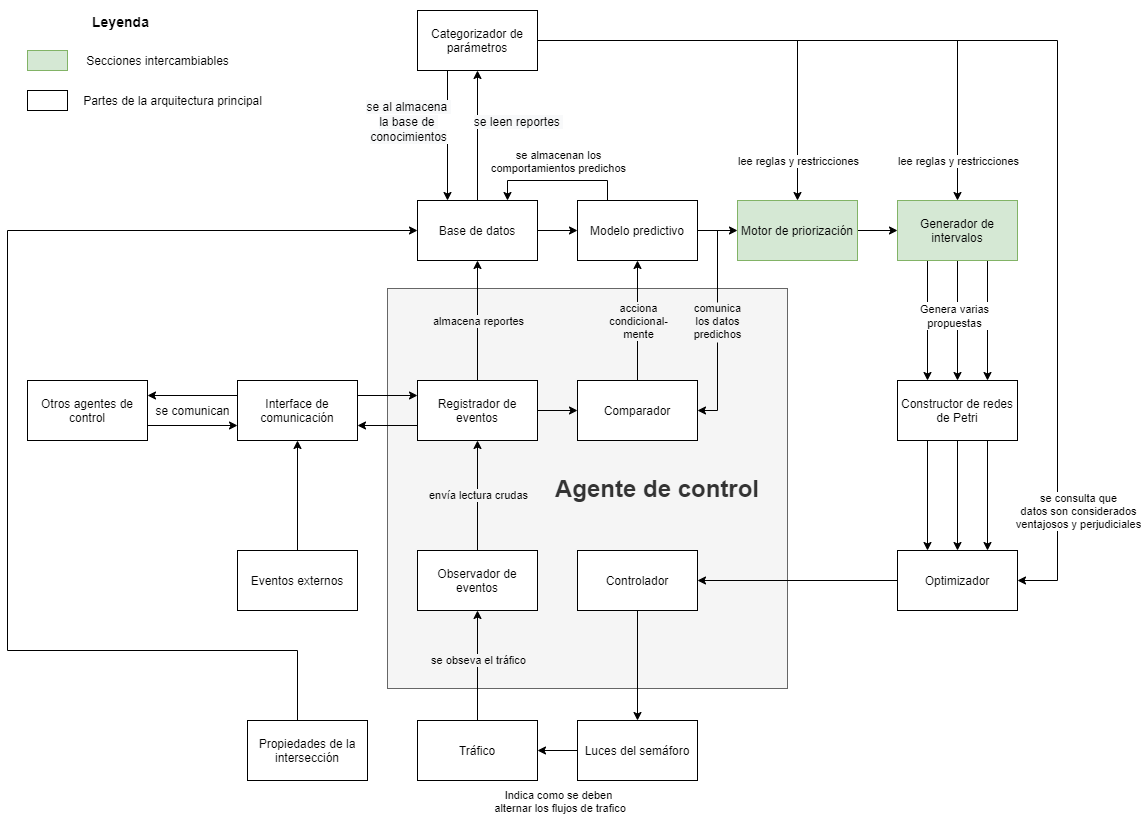
\includegraphics[width=\textwidth]{arquitectura.png} Fig. 1:
Arquitectura de un agente de control.

\hypertarget{truxe1fico}{%
\subsection{Tráfico}\label{truxe1fico}}

Los vehículos que se mueven en los carriles de la intersección y cruzan
de un carril a otro en nodos llamados intersecciones. Sobre las
intersecciónes puede haber ubicados semáforos.

\hypertarget{propiedades-de-la-intersecciuxf3n}{%
\subsection{Propiedades de la
intersección}\label{propiedades-de-la-intersecciuxf3n}}

Son las propiedades intrínsecas de la intersección que no suelen cambiar
con el paso del tiempo:

\begin{itemize}
\tightlist
\item
  Número de calles.
\item
  Carriles en cada calle.
\item
  Extensión aproximada de cada carril.
\item
  Estructura de la intersección: todas las posibles conexiones entre
  carriles.
\item
  Derechos y prioridades de paso.
\item
  Disposición de las luces del semáforo (cuántas hay y a que
  intersección apuntan).
\item
  Existencia de cruces y puentes peatonales, y si tienen algún botón que
  permita detener el tráfico.
\end{itemize}

\hypertarget{observador-de-eventos}{%
\subsection{Observador de eventos}\label{observador-de-eventos}}

Su única tarea es ser el sentido de la vista del agente de control.
Tiene funciones para observar eventos de interés que suceden con
regularidad en el mundo real en un momento dado y sus propiedades, tales
como:

\begin{itemize}
\tightlist
\item
  El paso de los vehículos, con propiedades como:

  \begin{itemize}
  \tightlist
  \item
    Ruta que toma (pueden seguir derecho o girar en algún sentido).
  \item
    Velocidad promedio aproximada.
  \item
    Cuanto tiempo permanece detenido.
  \item
    Aceleración aproximada.
  \end{itemize}
\item
  Cambios de luces (en que carril y a que color cambió).
\end{itemize}

Y también notifica eventos emergentes y sus propiedades, como:

\begin{itemize}
\tightlist
\item
  Aparición de un vehículos de prioridad (de que tipo y en que carril).
\item
  Un accidente (que carril obstruye).
\end{itemize}

Todo lo observado lo comunica al \emph{Registrador de eventos} indicando
el tiempo exacto en el que sucedió (\emph{timestamp}).

\hypertarget{registrador-de-eventos}{%
\subsection{Registrador de eventos}\label{registrador-de-eventos}}

Es el encargado de guardar un caché de los datos crudos enviados por el
\emph{Observador de eventos} e interpretarlos, para cada hora generar
reportes con datos derivados que se almacenan en la base de datos. El
reporte generado agrupa los datos por ciclo de semáforo, siendo éstos
los siguientes:

\begin{itemize}
\tightlist
\item
  Flujo por carril, es decir, el número de vehículos que pasan por cada
  carril cada determinado tiempo.
\item
  Tiempo de espera promedio por carril.
\item
  Densidad de cada carril.
\item
  Cola más larga en la señal roja.
\item
  Número de vehículos que pasan en señal verde.
\item
  Tiempo ocioso de la señal verde.
\item
  Cola más larga próxima fase.
\item
  Tiempo de cambio de la cola más larga en señal roja.
\end{itemize}

También recibe datos al exterior a través de la \emph{Interfaz de
comunicación}, que se almacenan selectivamente en la base de datos.

\hypertarget{interfaz-de-comunicaciuxf3n}{%
\subsection{Interfaz de
comunicación}\label{interfaz-de-comunicaciuxf3n}}

Permite enviar y recibir reportes de otros agentes de control, así como
notificaciones de eventos externos que pueden alterar el tráfico, como:

\begin{itemize}
\tightlist
\item
  Alertas de desastre natural.
\item
  Eventos públicos y días festivos.
\item
  Manifestaciones.
\end{itemize}

\hypertarget{comparador}{%
\subsection{Comparador}\label{comparador}}

Se encarga de comparar constantemente el comportamiento de los eventos
registrados con el comportamiento predicho. Cuando estos difieren de
manera significativa, el comparador solicita al \emph{Modelo predictivo}
que genere una nueva predicción. También se encarga de solicitar nuevas
predicciones cada que un evento externo lo solicite.

\hypertarget{modelo-predictivo}{%
\subsection{Modelo predictivo}\label{modelo-predictivo}}

Se alimenta del histórico de reportes generados por el \emph{Registrador
de eventos} que obtiene de la base de datos para predecir del
comportamiento de una intersección durante la siguiente hora. Los datos
que genera son los mismos que figuran el los reportes creados por el
\emph{Registrador de eventos}. También hace predicciones bajo demanda
cuando el \emph{Comparador} lo solicita.

\textbf{(Incluir aquí gráfica que represente el rango de tiempo en el
que son válidas las predicciones, la estimación de pérdida de tiempo
efectivo por el tiempo de generación, etc.)}

Ya que el proceso de hacer una predicción y su posterior optimización es
un proceso intensivo, las peticiones para nuevas predicciones suceden
cada hora, pero de manera escalonada. Por ejemplo: si existen 4 agentes
de control, uno iniciará una petición de predicción a las 2:00 p.m.,
mientras que otra los hará a las 2:15 p.m., otro a las 2:30, y así
sucesivamente, de tal manera que el tiempo entre cada hora se se reparta
lo más igualitariamente posible. De la mano con estas peticiones
escalonadas, las peticiones se realizarán de manera asíncrona usando
hilos de procesamiento para lograr paralelizar el procesamiento de
varias intersecciones a la vez de ser necesario. De esta manera, se
aprovecha también el sistema de encolamiento de hilos nativo de los
sistemas operativos, que resulta particularmente útil para no atrasar
las predicciones programadas por las realizadas bajo demanda.

\hypertarget{categorizador-de-paruxe1metros}{%
\subsection{Categorizador de
parámetros}\label{categorizador-de-paruxe1metros}}

Se encarga de categorizar la influencia de los parámetro predichos entre
sí mismos y como finalmente influyen sobre el comportamiento global del
tráfico, para así obtener conclusiones en forma de restricciones y
reglas aplicadas para al temporizado de los ciclos del semáforo.
Categoriza intervalos de tiempo que presentan una serie de condiciones a
términos abstractos, como: ``hora pico'', ``hora sin actividad'' o
``tráfico esporádico'', para así poder usar esas categorías como
condiciones para las reglas y restricciones vistas anteriormente.
Categoriza como ventajoso o perjudicial el incremento o decremento de un
parámetro respecto a parámetros que se busquen incrementar o decrementar
(como el tiempo de espera, la generación de colas, etc). De ser
necesario, infiere una función de como su variación afecta a estos
parámetros.

Ejemplo verbal: si se hacen ciclos en verde un un carril \textbf{mayores
a} 45 segundos durante \textbf{horas pico}, se genera una \textbf{cola
de espera perjudicial a la fluidez} del carril perpendicular, entonces
se infiere una regla que impida que se rebase ese tiempo de ciclo dadas
esas condiciones, y en caso de que se tenga que se rebase, se tenga la
función que indica que tanto perjudica ese aumento para calcular los
tiempos de ciclo que produzcan el mejor costo-beneficio (pues se tienen
que tomar en cuenta el resto de los parámetros).

Este módulo analiza constantemente los reportes almacenados en la base
de datos para realizar el proceso mencionado anteriormente y todo lo
inferido se guarda de manera centralizada como una base de conocimientos
central como registros en la base de datos.

Este módulo se inspiro en la llamada \emph{Colección de hechos} usada en
\textcite{JoelTrejo2006}.

\begin{quote}
La colección de hechos alberga los datos correspondientes a la
aplicación de determinada estrategia de control cuando se presentan
ciertas condiciones en el tráfico observado. La colección de hechos
puede desempeñar el papel de memoria auxiliar en la cual se registran
los razonamientos llevados a cabo. \textcite[p. 47]{JoelTrejo2006}
\end{quote}

\hypertarget{motor-de-priorizaciuxf3n}{%
\subsection{Motor de priorización}\label{motor-de-priorizaciuxf3n}}

Se encarga de asignar un valor numérico a cada carril, que indica su
prioridad. Entre mayor el número, mayor la prioridad. Este número de
genera usando como base la demanda predicha, aunque también es posible
usar restricciones y reglas definidas por el \emph{Categorizador de
parámetros}.

\hypertarget{generador-de-intervalos}{%
\subsection{Generador de intervalos}\label{generador-de-intervalos}}

Usa los valores generados por el \emph{Motor de priorización} para
generar una proporción de la duración de cada fase del semáforo en la
duración total del ciclo. Posteriormente usa como base las reglas y
restricciones generados por el \emph{Categorizador de parámetros} para
generar varias propuestas de la duración total del ciclo de fases de
luces. Se obtiene como salida varios juegos de propuestas de duraciones
de fases que pueden haber tomado en cuenta diferentes reglas.

\hypertarget{constructor-de-redes-de-petri}{%
\subsection{Constructor de redes de
Petri}\label{constructor-de-redes-de-petri}}

A partir de las propuestas de intervalos generadas por el
\emph{Generador de intervalos}, se encarga de construir una red de Petri
temporizada para cada una de ellas.

\hypertarget{optimizador}{%
\subsection{Optimizador}\label{optimizador}}

Recibe múltiples propuestas de redes de Petri y a través de algoritmos
genéticos, cruza los genes de las diferentes propuestas (que tomaron en
cuenta diferente reglas para construirse) buscando maximizar los
parámetros considerados como ventajosos (como el flujo) y minimizar los
considerados como perjudiciales (como las cosas y los tiempos de
espera). La información de cuáles son estos parámetros se obtiene del
\emph{Categorizador de parámetros}. Al final da como salida una red de
Petri optimizada.

\hypertarget{controlador}{%
\subsection{Controlador}\label{controlador}}

Tiene las funciones para necesarias para leer la red de Petri
temporizada que recibe y controlar los cambios de luces según lo indique
la red.

\hypertarget{luces-de-semuxe1foro}{%
\subsection{Luces de semáforo}\label{luces-de-semuxe1foro}}

Son la manera en la que se plasman los intervalos de luces generados y
son lo que físicamente indica a los conductores cuando deben circular o
detenerse.

\clearpage % Nueva página
